No. of passengers=3000,\\
End\_sim\_time = 5000,\\
getSpottingsNowTime = 2000,\\
peakThres=5 (500 meters both sides)\\
PosConf calculated for each point at distance of= 100 meters\\
Starting time gap between trains=8.33 min (500 sec)\\
Halt\_time\_of\_Train = 20 sec\\
Speed\_of\_The\_Train = 14 m/sec (50.4 km/h)\\

\subsection{With no of trains=1 }
\begin{figure}[h!]
\begin{minipage}{.5\textwidth}

\centering
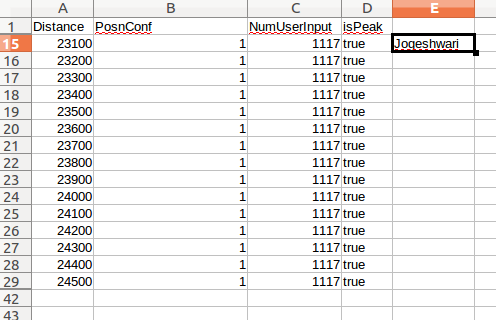
\includegraphics[height=6cm,width=9cm]{1_pre.png}
\caption{Predicted positions of the trains}

\end{minipage}%
\begin{minipage}{.5\textwidth}

\centering
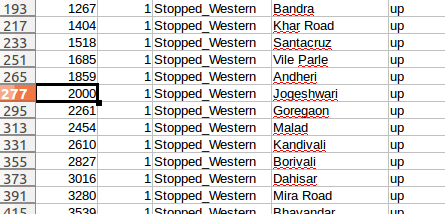
\includegraphics[height=5cm,width=8cm]{1_ori.png}
\caption{Real positions of the trains}

\end{minipage}%
\end{figure}
\subsection{With no of trains=2 }
\begin{figure}[h!]
\begin{minipage}{.5\textwidth}

\label{No of trains=2}
\centering
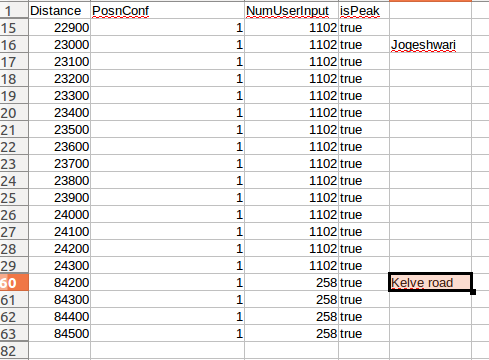
\includegraphics[height=6cm,width=9cm]{2_pre.png}
\caption{Predicted positions of the trains}

\end{minipage}%
\begin{minipage}{.5\textwidth}

\centering
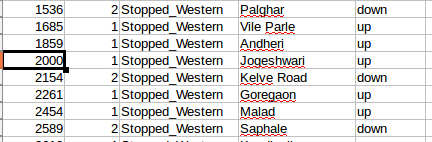
\includegraphics[height=5cm,width=8cm]{2_ori.png}
\caption{Real positions of the trains}

\end{minipage}%
\end{figure}
\subsection{With no of trains=3 }
\begin{figure}[h!]
\begin{minipage}{.5\textwidth}

\centering
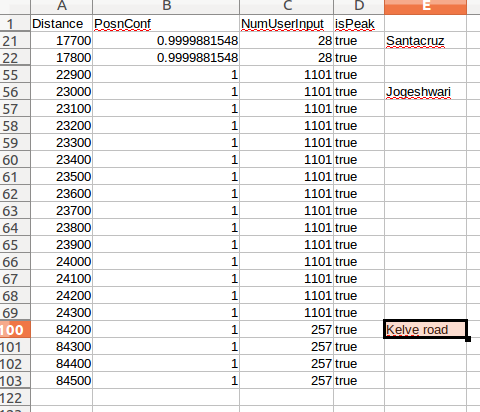
\includegraphics[height=6cm,width=9cm]{3_pre.png}
\caption{Predicted positions of the trains}

\end{minipage}%
\begin{minipage}{.5\textwidth}


\centering
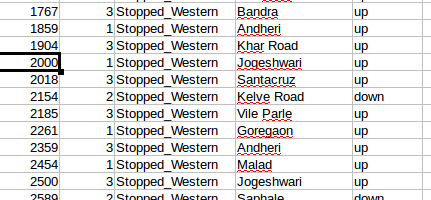
\includegraphics[height=5cm,width=8cm]{3_ori.png}
\caption{Real positions of the trains}

\end{minipage}%
\end{figure}
\subsection{With no of trains=4 }
\begin{figure}[h!]
\begin{minipage}{.5\textwidth}


\centering
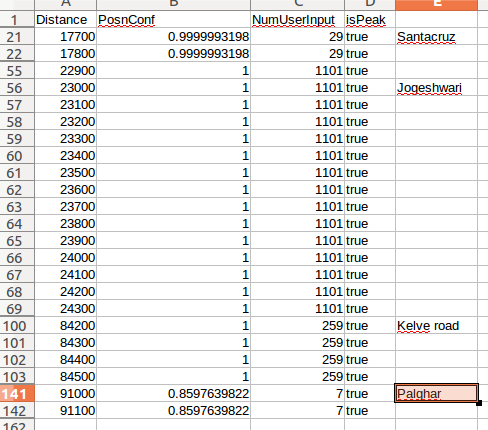
\includegraphics[height=6cm,width=9cm]{4_pre.png}
\caption{Predicted positions of the trains}

\end{minipage}%
\begin{minipage}{.5\textwidth}

\centering
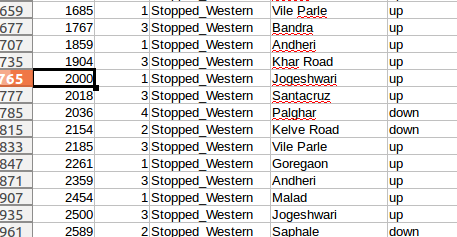
\includegraphics[height=5cm,width=8cm]{4_ori.png}
\caption{Real positions of the trains}

\end{minipage}%
\end{figure}
\newpage
\subsection{With no of trains=5 }
\begin{figure}[h!]
\begin{minipage}{.5\textwidth}

\centering
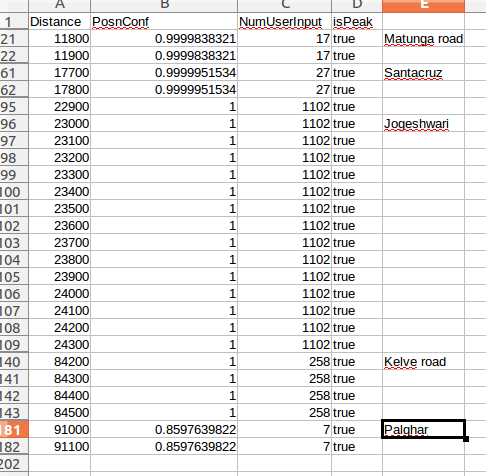
\includegraphics[height=6cm,width=9cm]{5_pre.png}
\caption{Predicted positions of the trains}

\end{minipage}%
\begin{minipage}{.5\textwidth}

\label{No of trains=1}
\centering
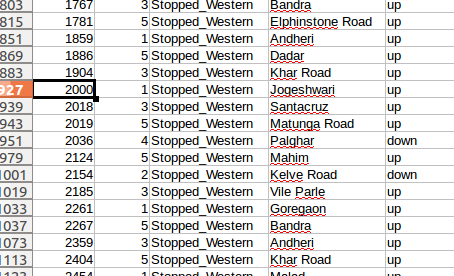
\includegraphics[height=5cm,width=8cm]{5_ori.png}
\caption{Real positions of the trains}

\end{minipage}%
\end{figure}

\subsection{With no of trains=6 }
\begin{figure}[h!]
\begin{minipage}{.5\textwidth}

\centering
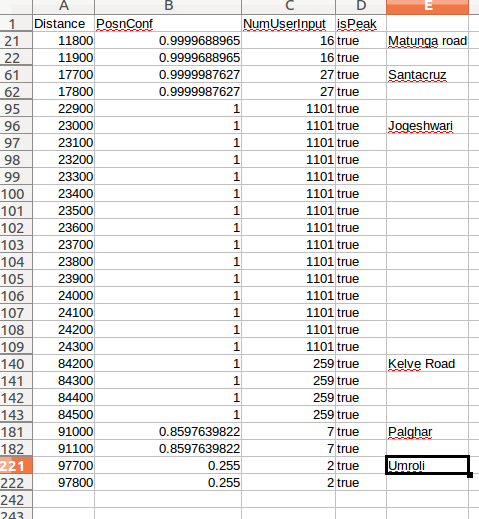
\includegraphics[height=6cm,width=9cm]{6_pre.png}
\caption{Predicted positions of the trains}

\end{minipage}%
\begin{minipage}{.5\textwidth}

\centering
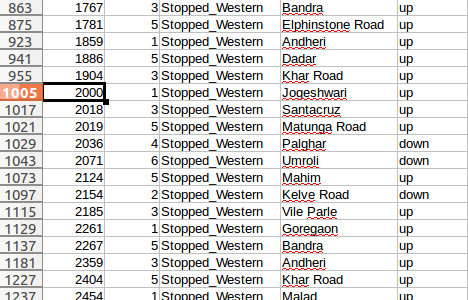
\includegraphics[height=5cm,width=8cm]{6_ori.png}
\caption{Real positions of the trains}

\end{minipage}%
\end{figure}
\newpage
\subsection{With no of passengers= 100000 and no of trains=5 }
\begin{figure}[h!]
\begin{minipage}{.5\textwidth}

\centering
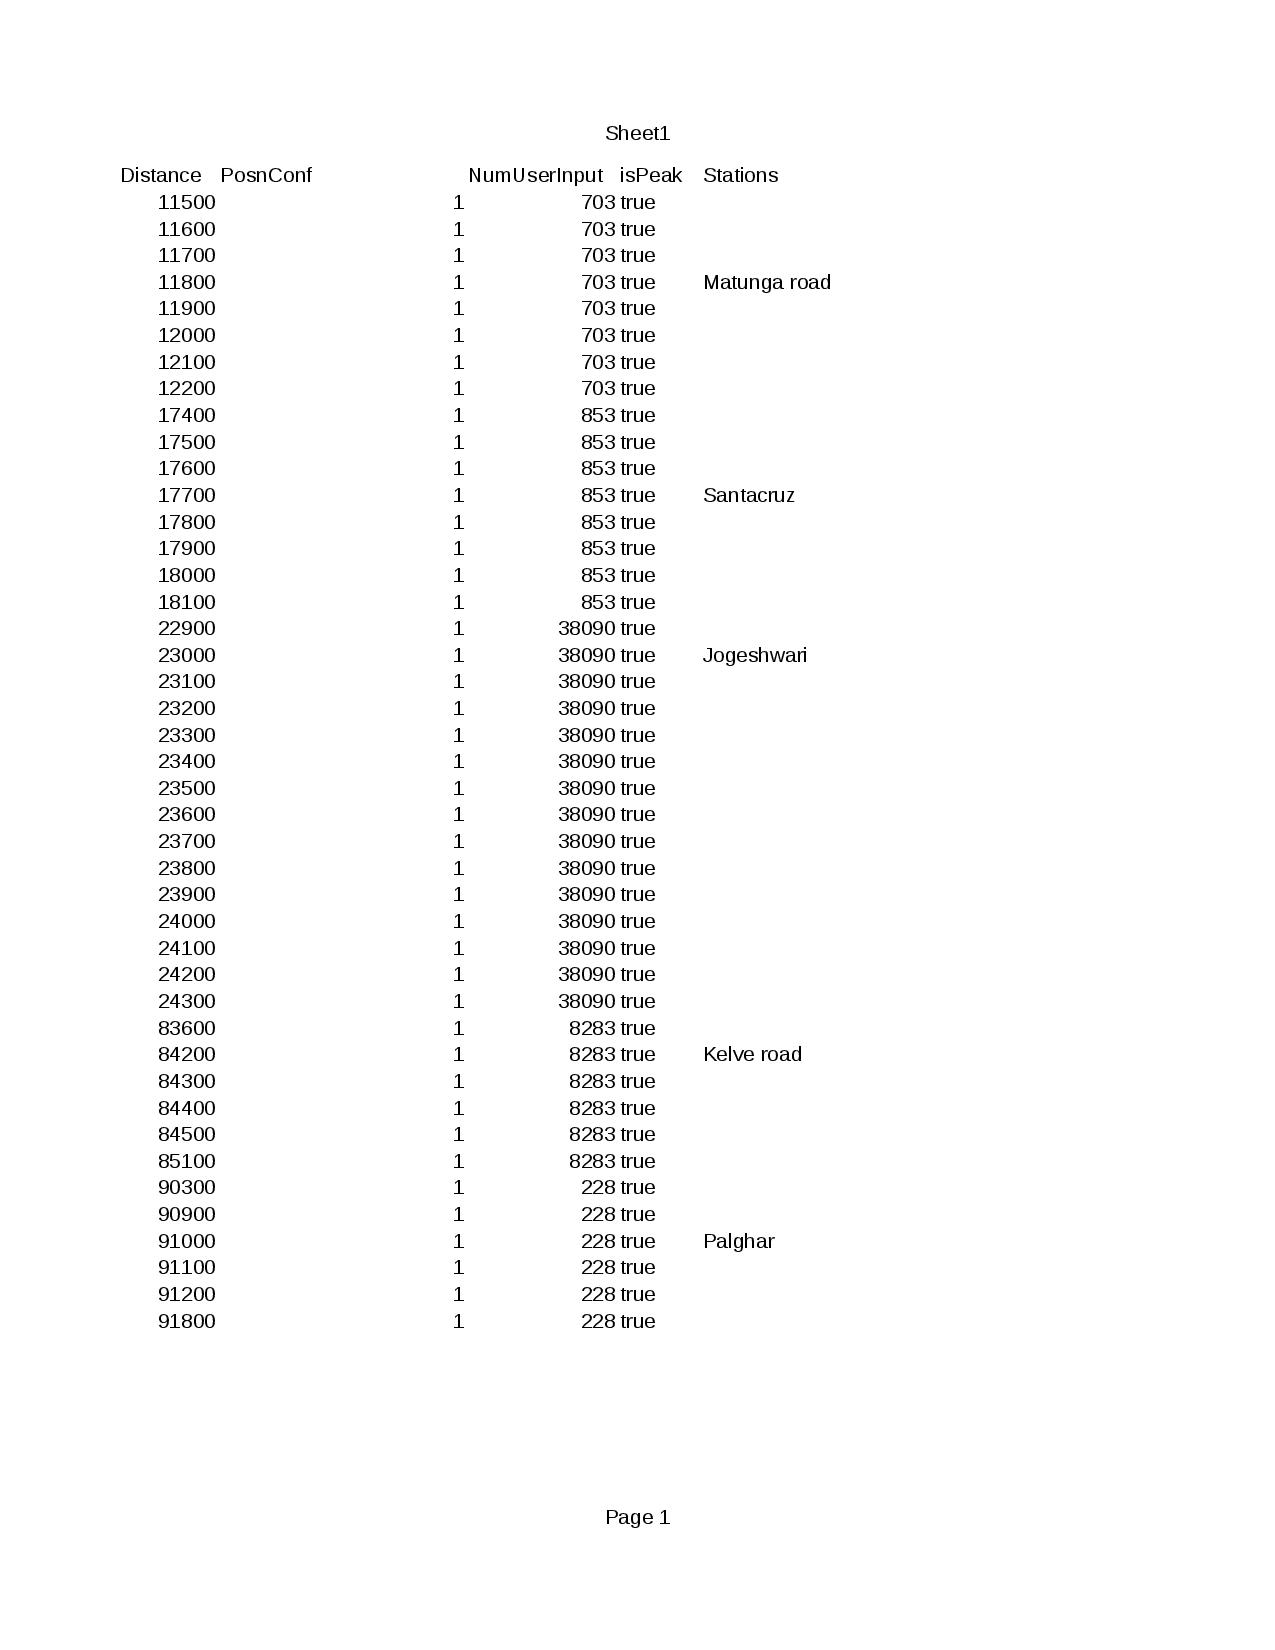
\includegraphics[height=17cm,width=13cm]{100000_User.jpg}
\caption{Predicted positions of the trains with 100000 passengers}

\end{minipage}%
\begin{minipage}{.5\textwidth}

\centering
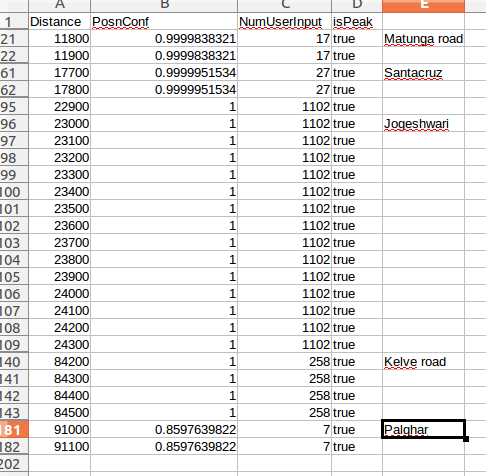
\includegraphics[height=7cm,width=8cm]{5_pre.png}
\caption{Predicted positions of the trains with 3000 users}

\end{minipage}%
\end{figure}

\newpage
\subsection{With no of passengers= 100000 and no of trains=10 }
\begin{figure}[h!]

\centering
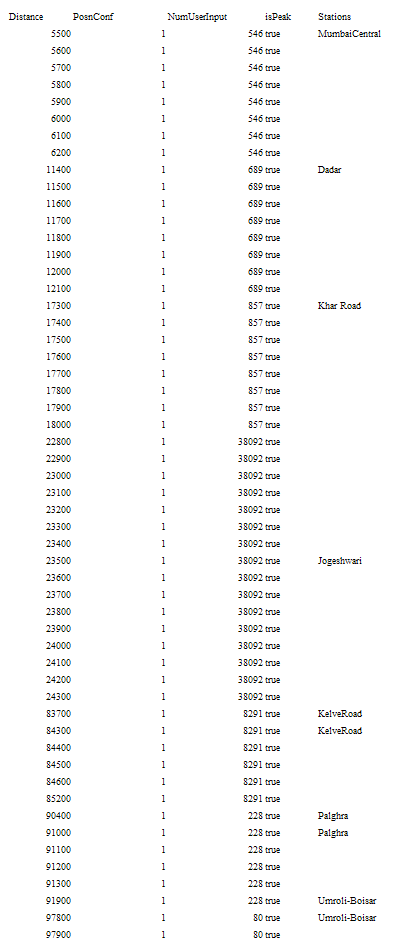
\includegraphics[height=20cm,width=18cm]{100000usr_10train.png}
\caption{Predicted positions of the trains with 100000 passengers}

\end{figure}

\newpage
\subsection{With no of passengers= 500000 and no of trains=10 }
\begin{figure}[h!]

\centering
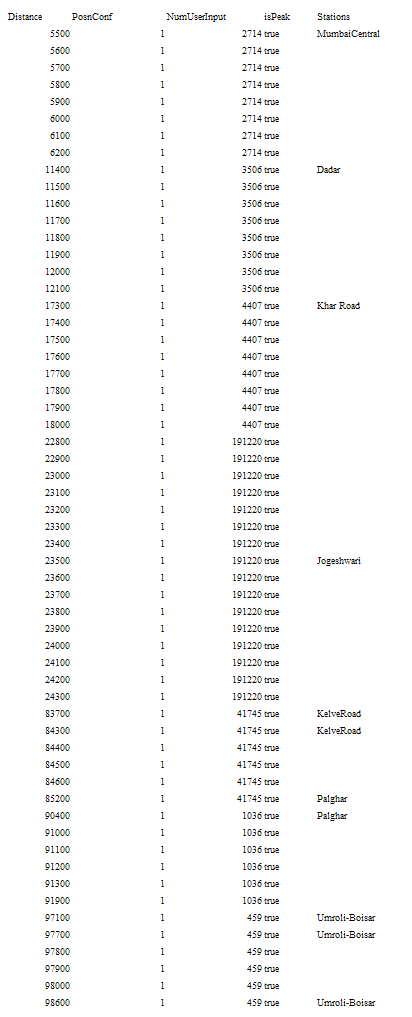
\includegraphics[height=20cm,width=18cm]{500000usr_10train.png}
\caption{Predicted positions of the trains with 500000 passengers}

\end{figure}






